%% LaTeX2e class for student theses
%% sections/methodology.tex
%% 
%% Karlsruhe Institute of Technology
%% Institute for Program Structures and Data Organization
%% Chair for Software Design and Quality (SDQ)
%%
%% Dr.-Ing. Erik Burger
%% burger@kit.edu
%%
%% Version 1.3.2, 2017-08-01

\chapter{Methodology}
\label{ch:Methodology}
The approach to developing an automatic system capable of procedures administered by EMS personnel consists of breaking the procedures into anatomical movements, developing an algorithm, and collecting data to train the algorithm through a user study. This thesis focuses on automatically detecting five EMS procedures performed inside an ambulance: placing a intravenous tourniquet, wrapping a wound, applying a bag-valve-mask, placing an oral airway, and \gls{CPR} (Figure \ref{fig:EMS-procedures}). The five EMS procedures were chosen for their reproducibility on a demo mannequin and their assumed recognition difficulty. CPR is assumed to be easily recognizable, due to the repetitive motion during compressions in the accelerometer data. Bag-valve-mask application is assumed to be easily recognizable, due to the repetitive motion during squeezing the bag in the EMG data. Placing a tourniquet is assumed to be harder to recognize, due to missing repetitive motion. Wrapping a wound is assumed to be harder to recognize, due to missing repetitive motion. Placing an oral airway is assumed to be the hardest to recognize, due to missing repetitive motion and a short duration. 
\begin{figure}[b]
	\centering
	\begin{subfigure}[b]{0.18\textwidth}
		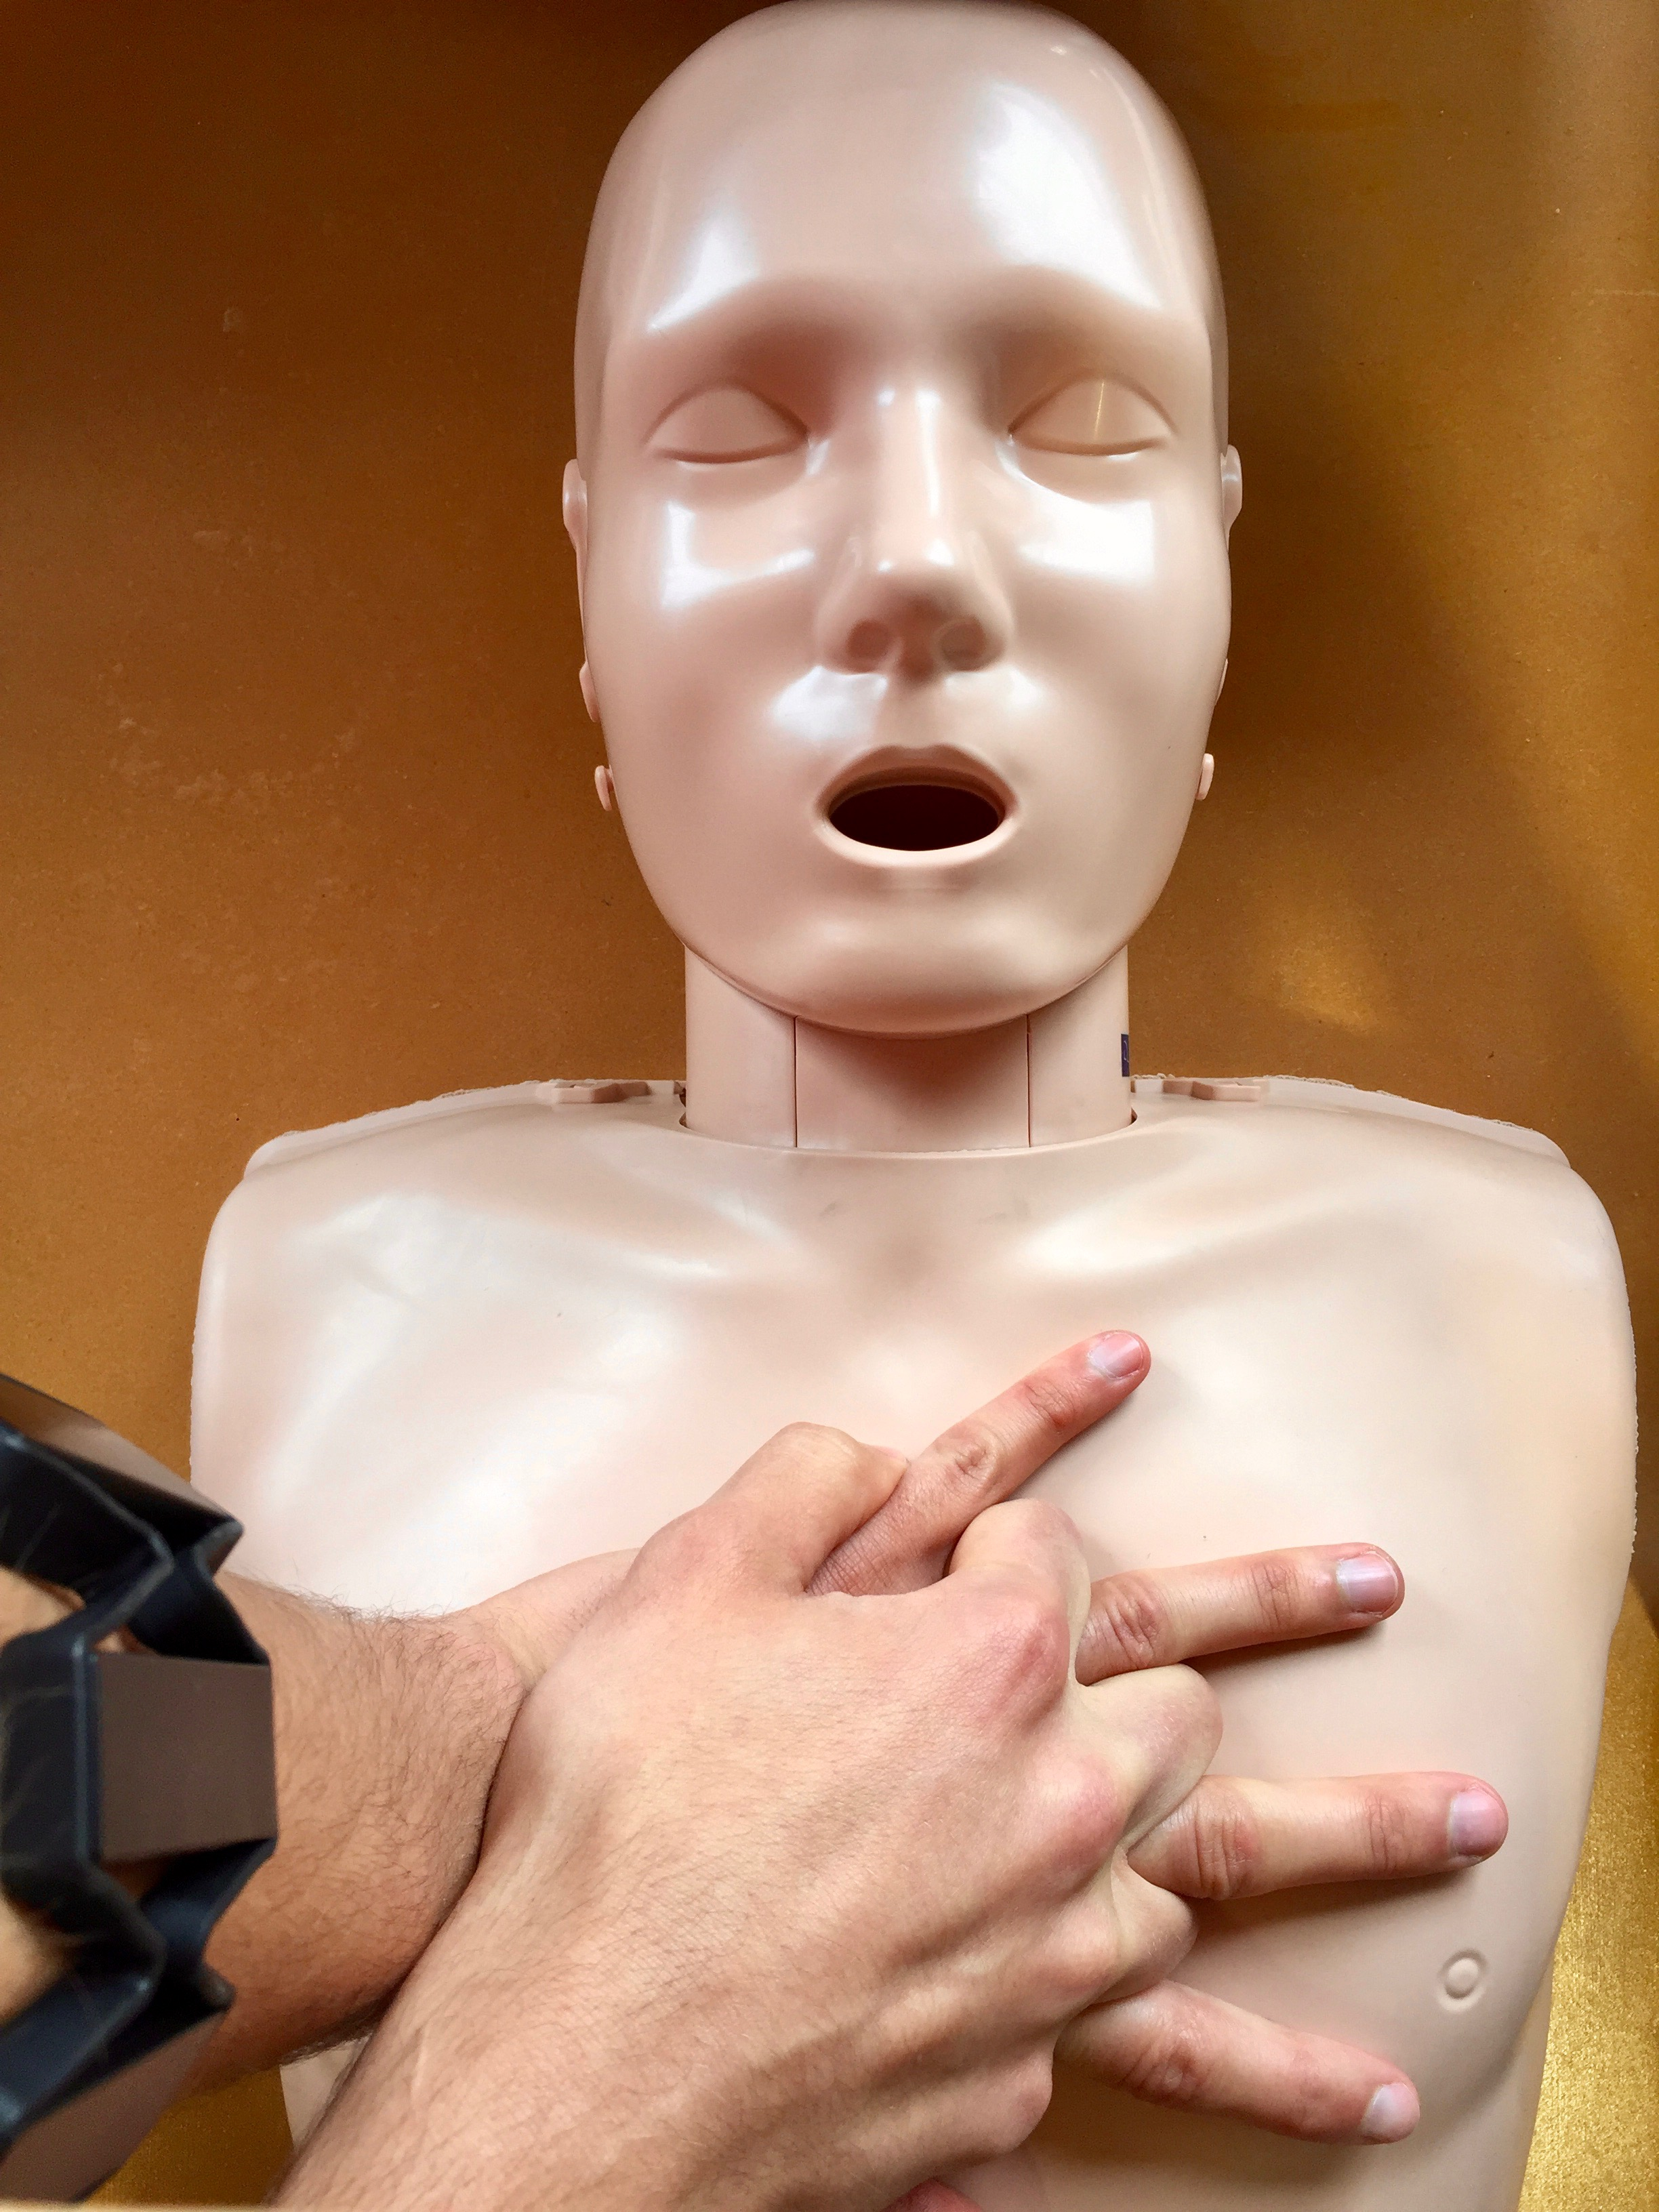
\includegraphics[width=\textwidth]{pictures/cpr}
		\caption{CPR}
		\label{fig:cpr}
	\end{subfigure}
	~ %add desired spacing between images, e. g. ~, \quad, \qquad, \hfill etc. 
	%(or a blank line to force the subfigure onto a new line)
	\begin{subfigure}[b]{0.18\textwidth}
		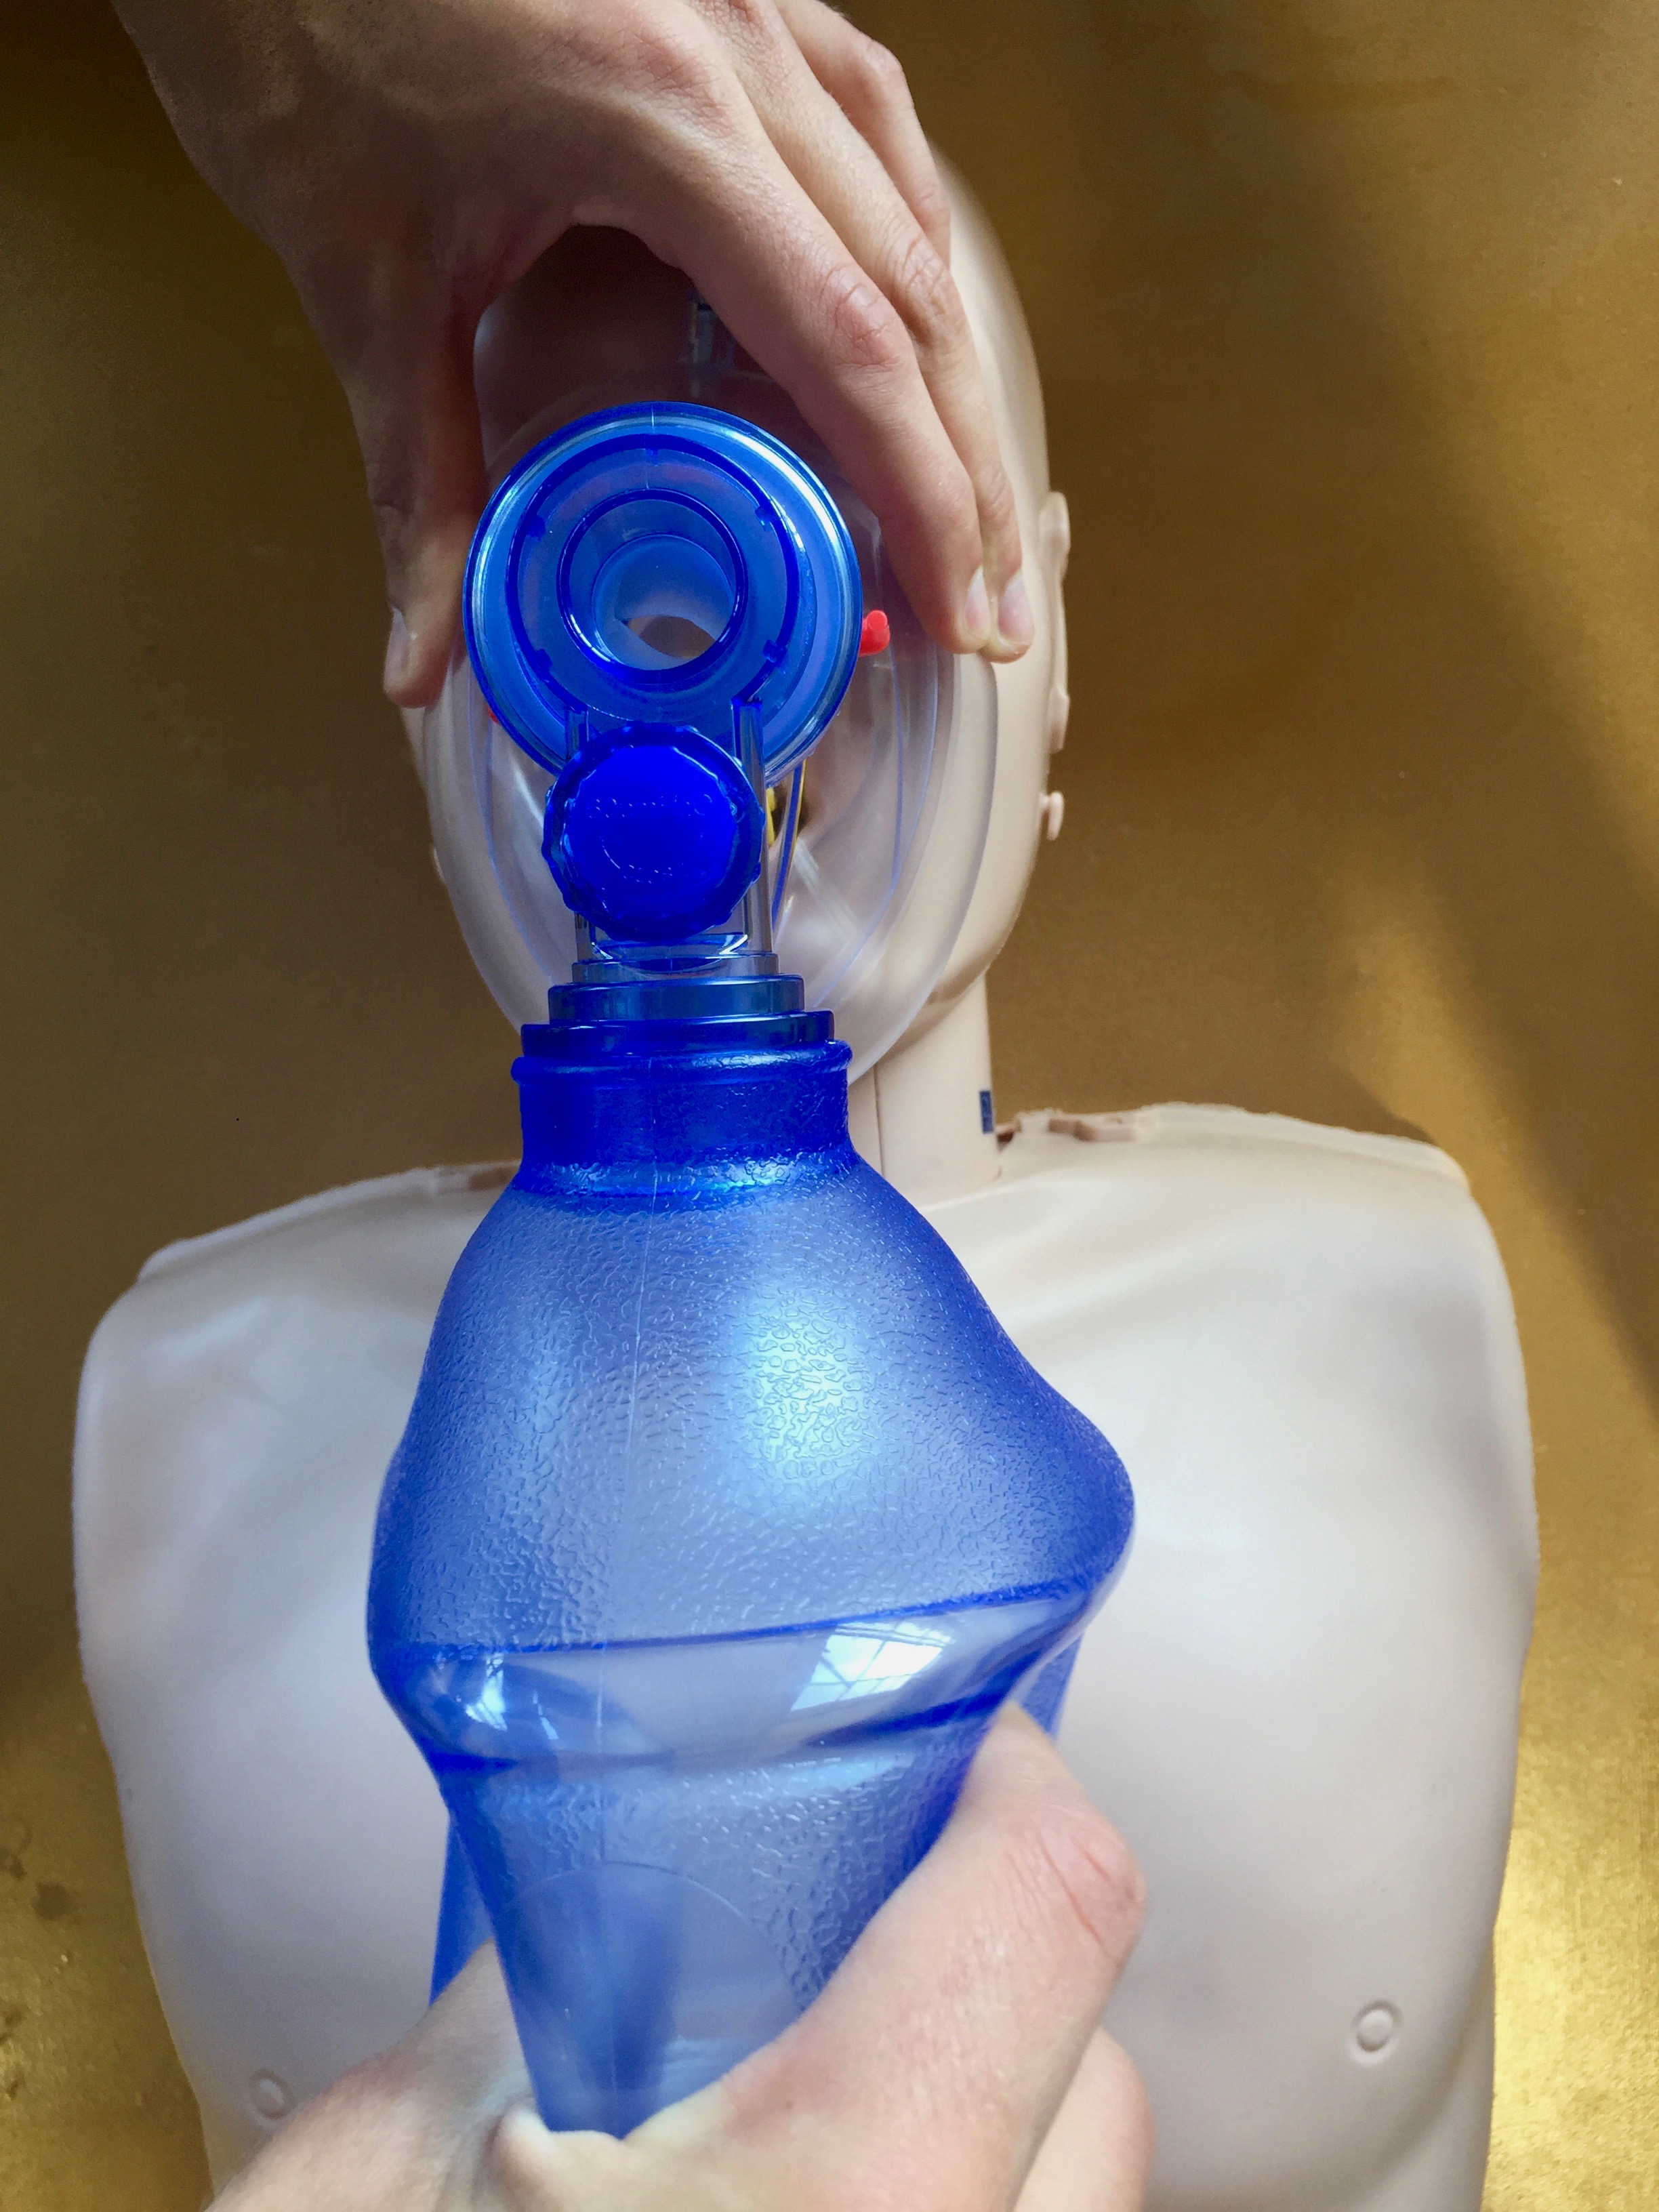
\includegraphics[width=\textwidth]{pictures/bagging}
		\caption{Bagging}
		\label{fig:bagging}
	\end{subfigure}
	~ %add desired spacing between images, e. g. ~, \quad, \qquad, \hfill etc. 
	%(or a blank line to force the subfigure onto a new line)
	\begin{subfigure}[b]{0.18\textwidth}
		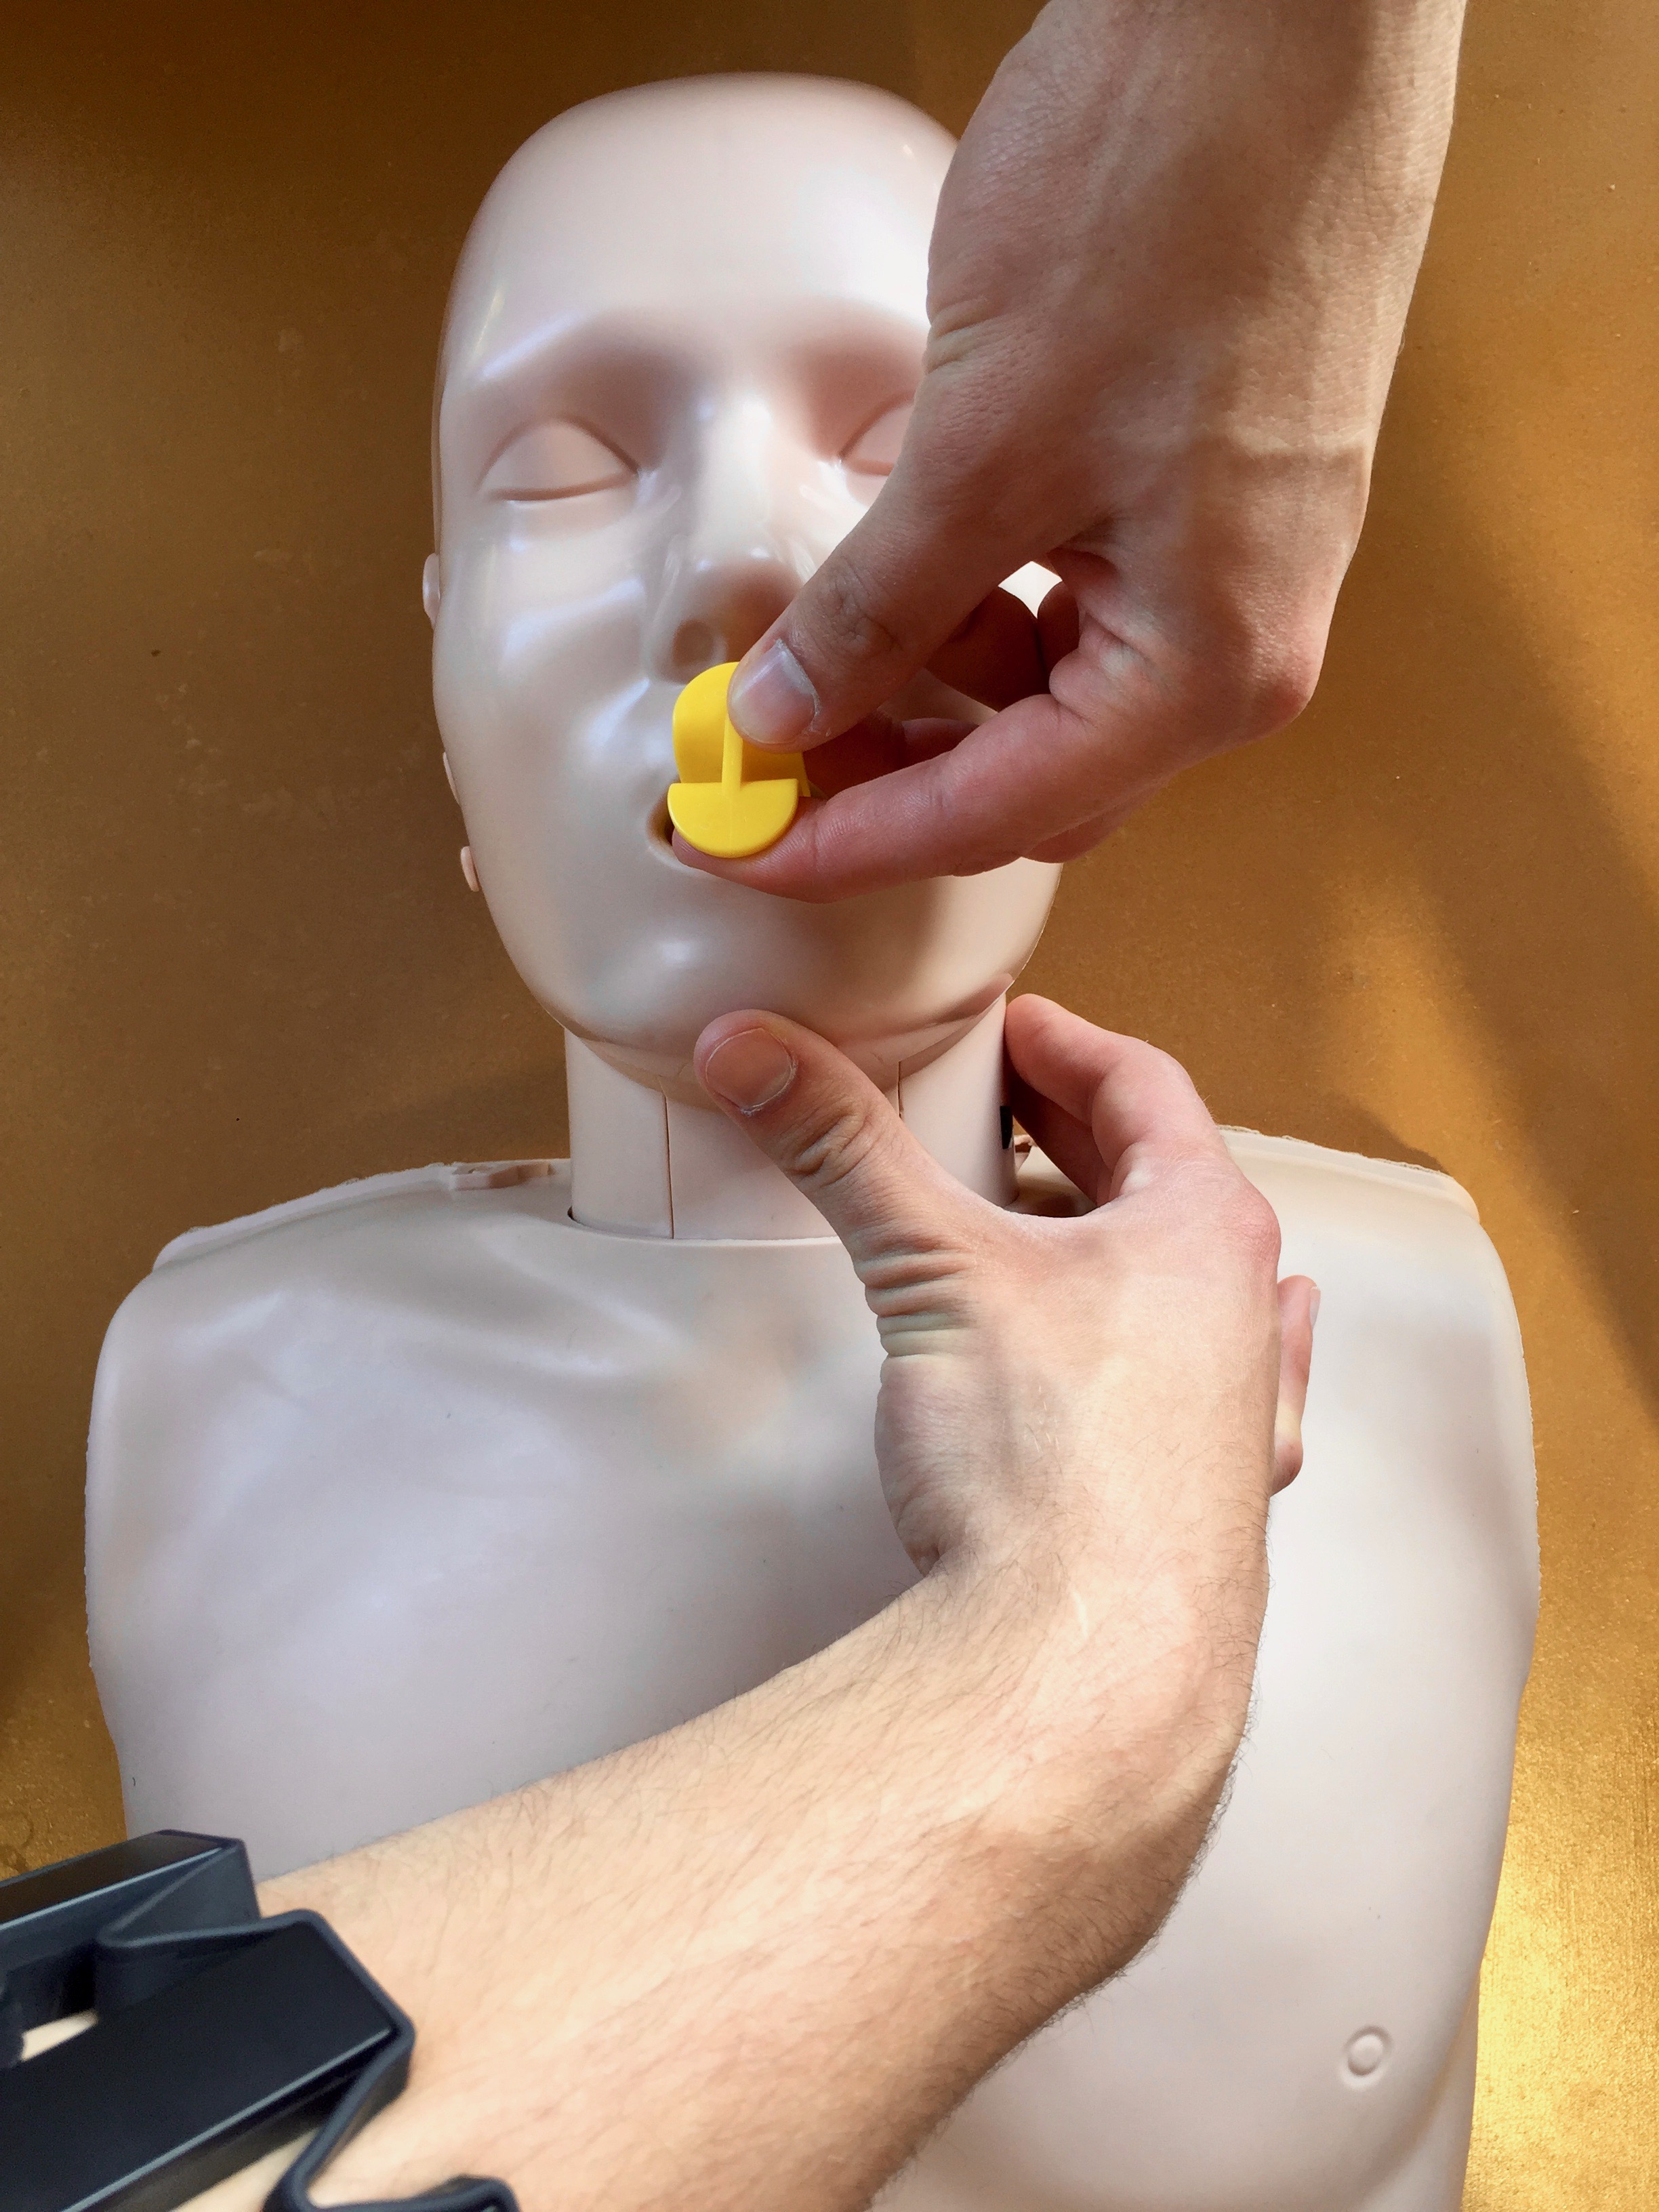
\includegraphics[width=\textwidth]{pictures/oral-airway}
		\caption{Airway}
		\label{fig:oral-airway}
	\end{subfigure}
	~ %add desired spacing between images, e. g. ~, \quad, \qquad, \hfill etc. 
	%(or a blank line to force the subfigure onto a new line)
	\begin{subfigure}[b]{0.18\textwidth}
		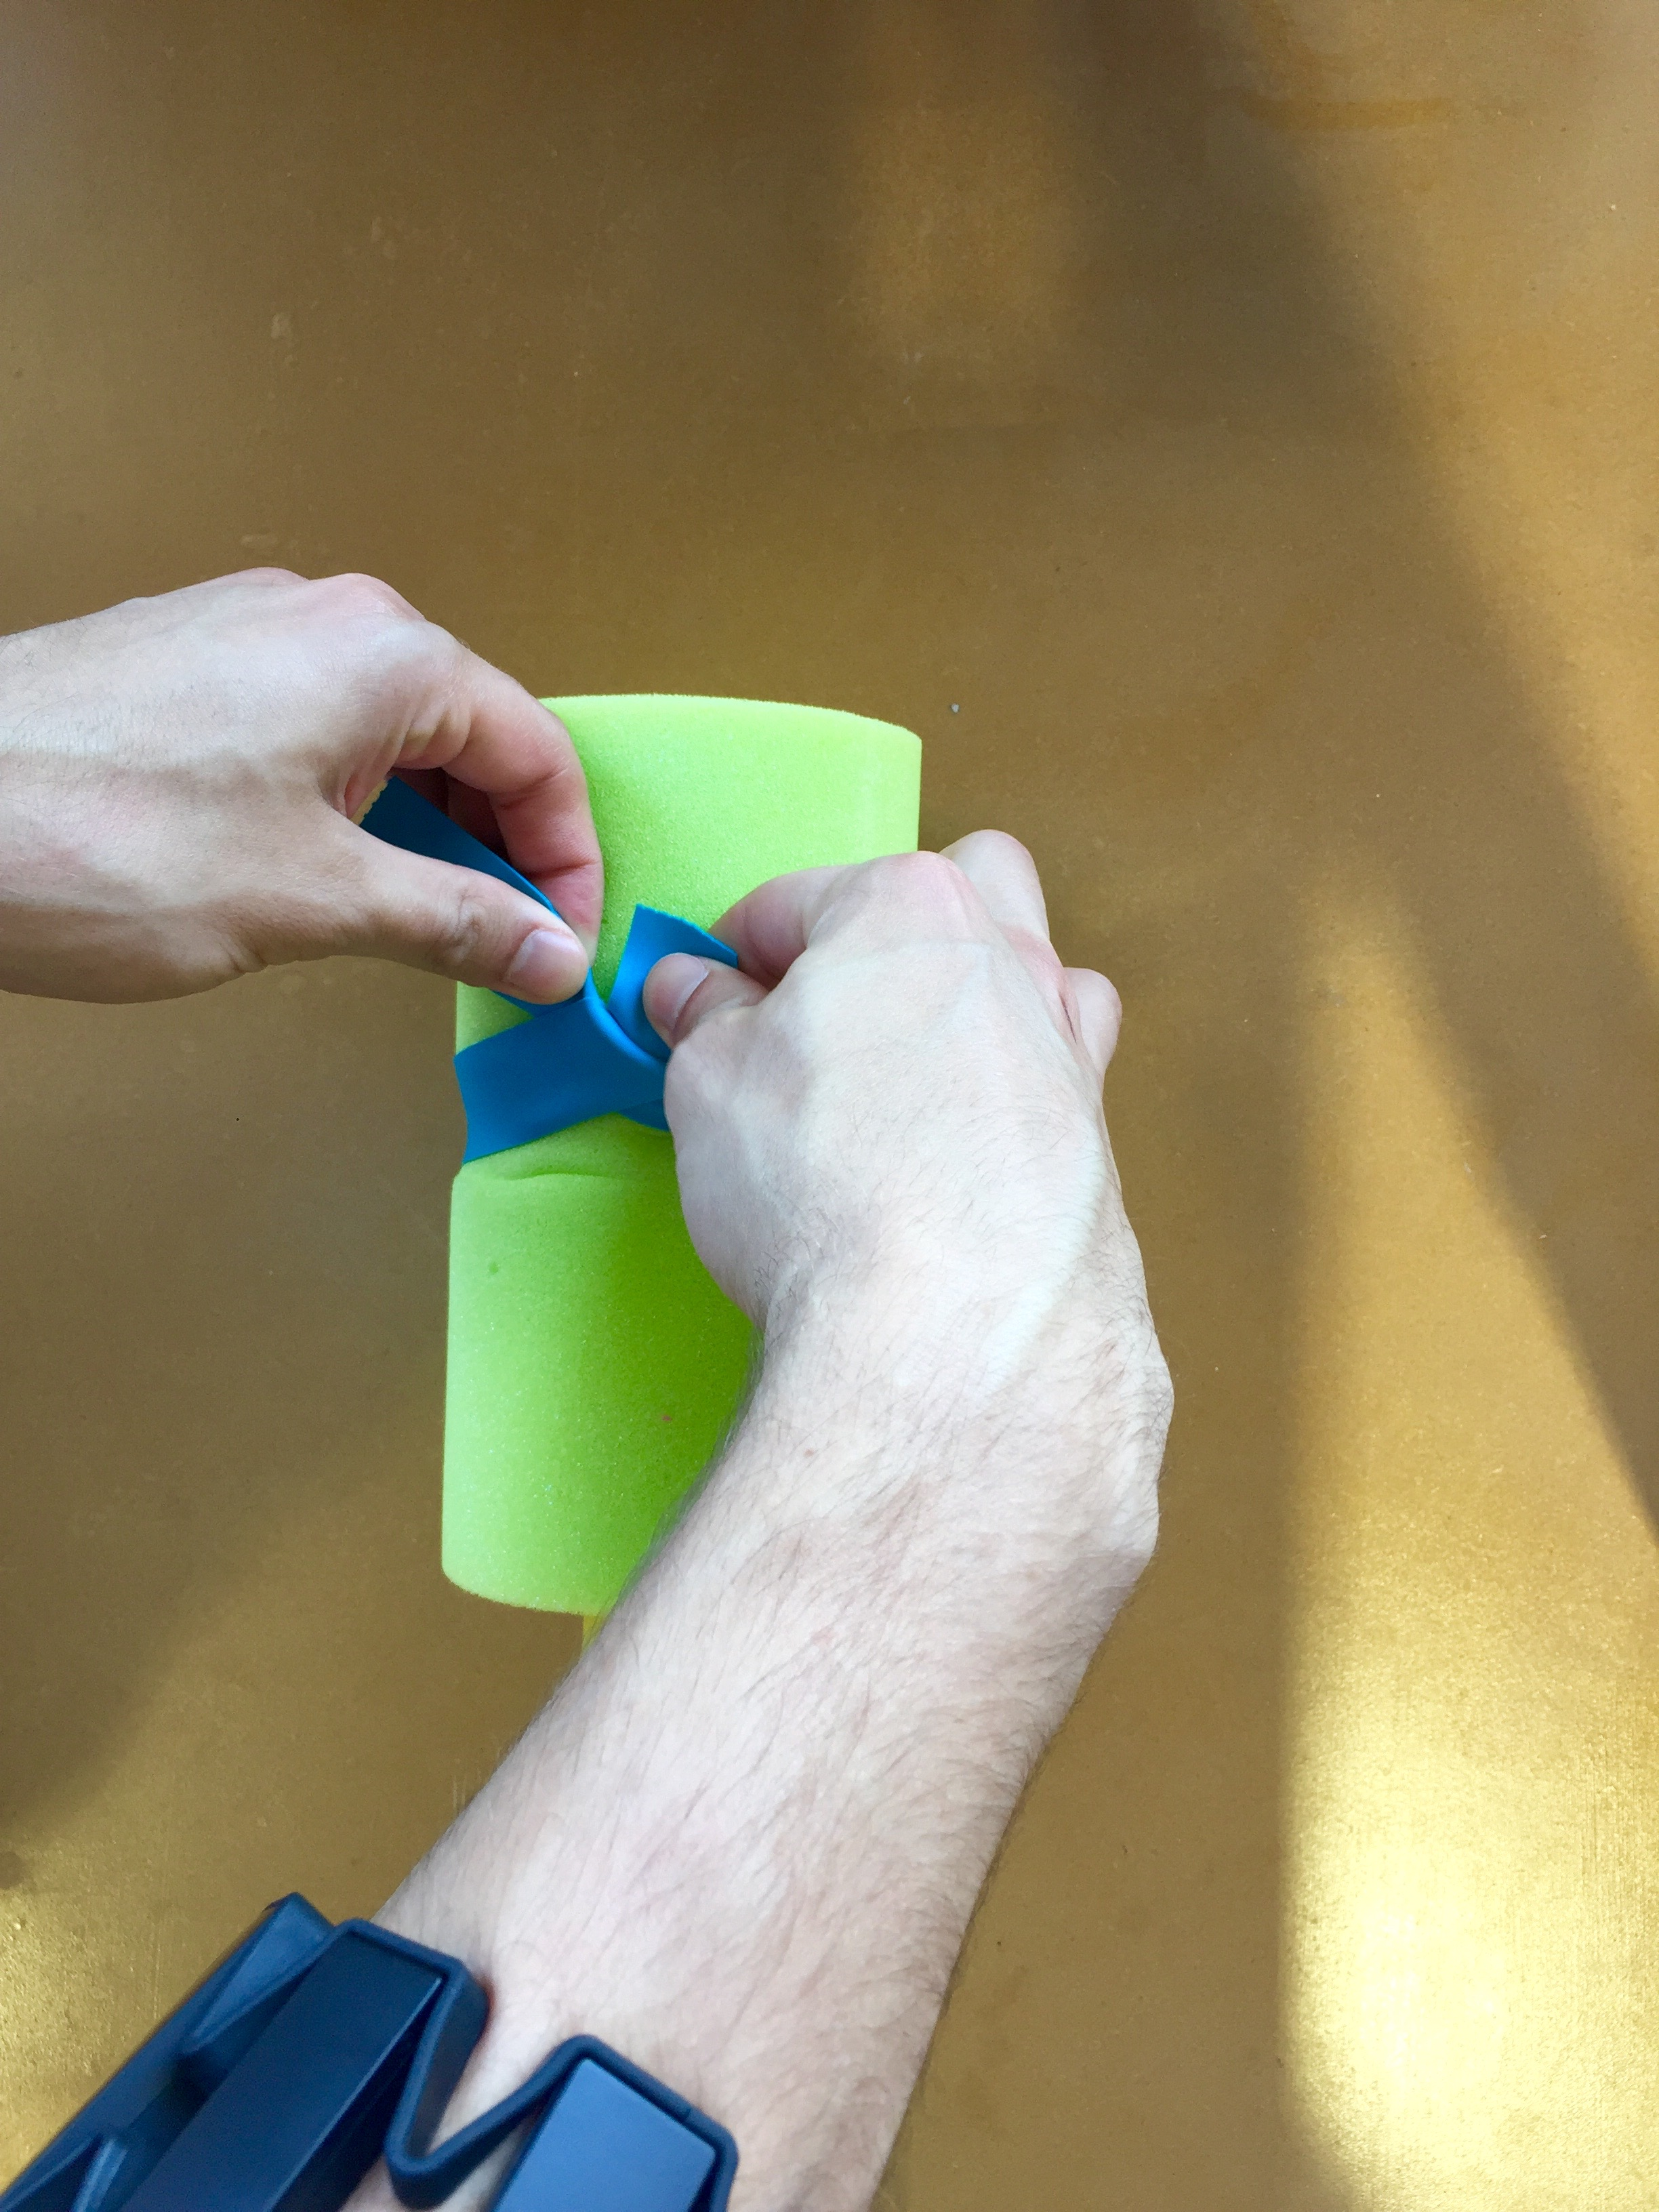
\includegraphics[width=\textwidth]{pictures/tourniquet}
		\caption{Tourniquet}
		\label{fig:tourniquet}
	\end{subfigure}
	~ %add desired spacing between images, e. g. ~, \quad, \qquad, \hfill etc. 
	%(or a blank line to force the subfigure onto a new line)
	\begin{subfigure}[b]{0.18\textwidth}
		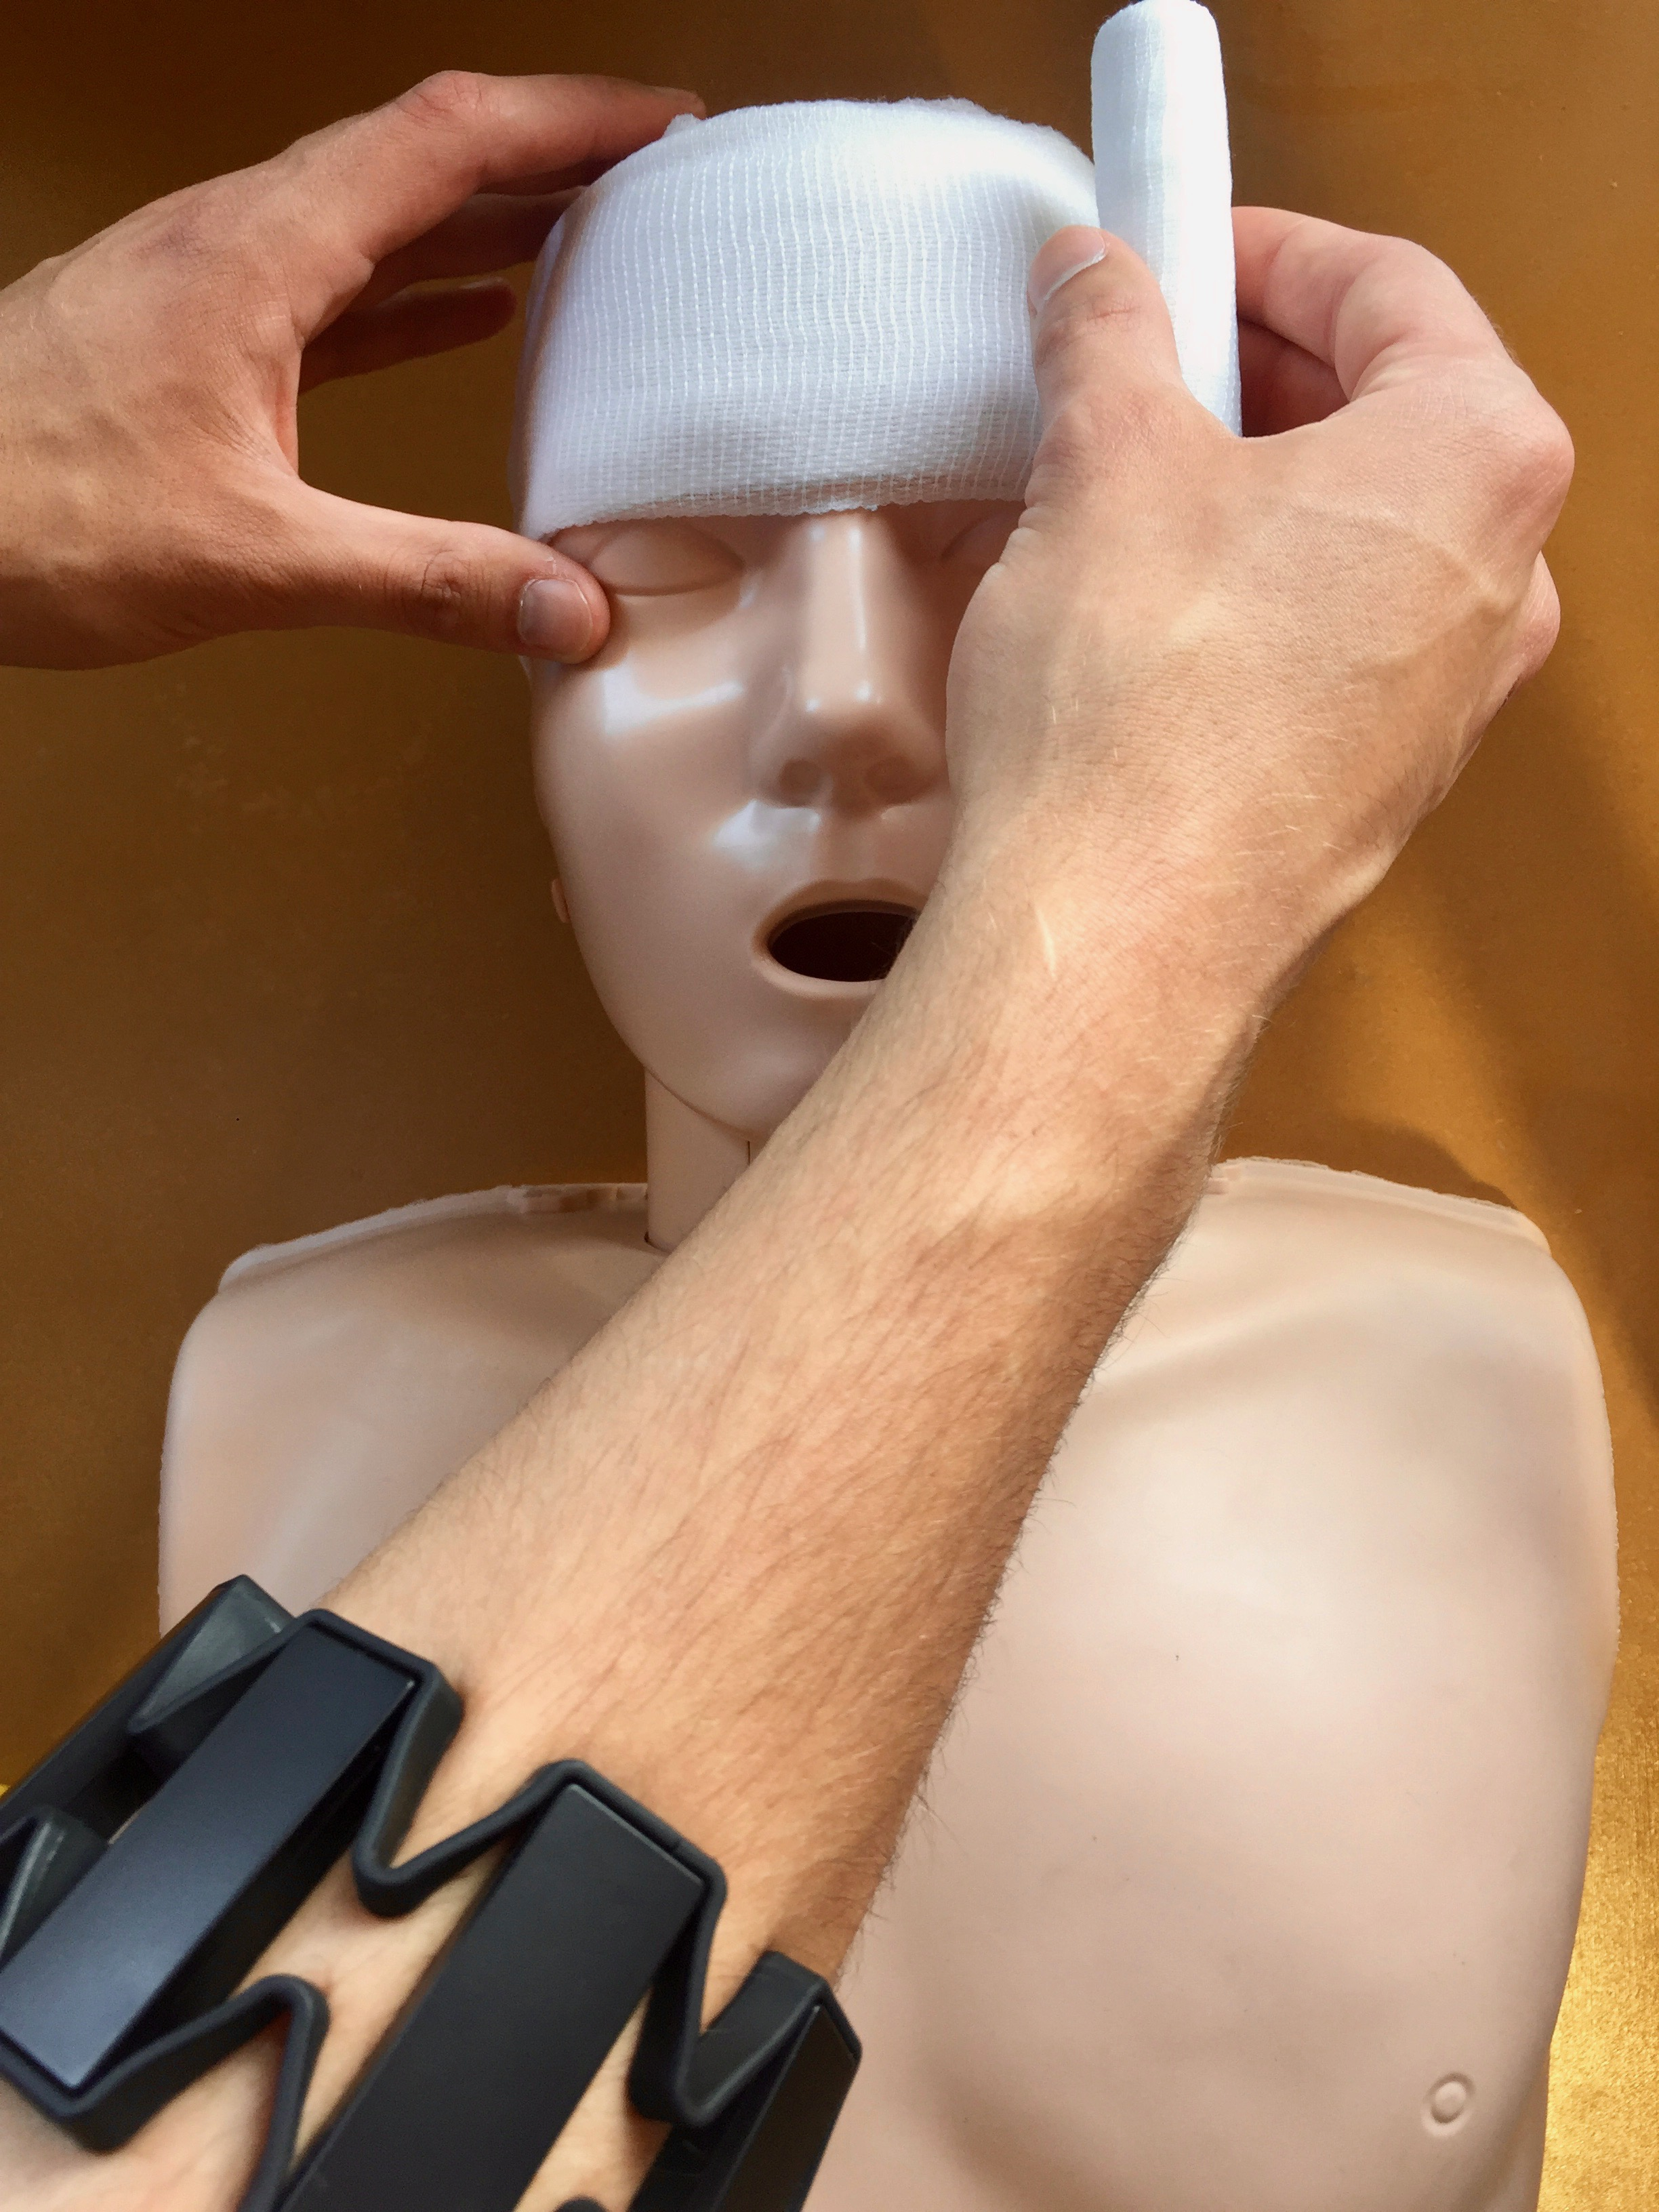
\includegraphics[width=\textwidth]{pictures/wound}
		\caption{Wound}
		\label{fig:wound}
	\end{subfigure}
	\caption{EMS procedures}
	\label{fig:EMS-procedures}
\end{figure}
\section{Hierarchical Task Analysis}
\label{sec:Approach:Hierarchical-Task-Analysis}
Medical procedures include repetitive and unique movements. Distinctive patterns in the data from repetitive and unique movements help machine-learning algorithms achieve higher performance. Therefore, the EMS procedures are broken into their anatomical movements using \emph{Hierarchical Task Analysis} in order to identify distinctive patterns in the EMS procedures \cite{kirwan1992guide}. The Hierarchical Task Analysis divides tasks (procedures) into sub-tasks, followed by sub-sub-tasks, and finally anatomical movements. The resulting anatomical movements are analyzed to include their sensability using five commercially available sensors: Apple Watch, Myo, Empatic E4, Garmin Watch Forerunner, and Bioharness BT. Sensability is the ability of a sensor to recognize a human movement. The sensability is determined by considering the type of sensor data and the sensors' ability to detect anatomical movements, such as recognizing muscle movement through EMG data. The placement of a sensor is crucial in its ability to detect anatomical movements. The EMG data for the hand is captured by placing the sensor on the arm. Table \ref{tab:hta:overview} displays an overview of the procedures with their respective sensability per sensor.
\par CPR is a procedure that is performed on patients with cardiac arrest to preserve brain functionality. The Hierarchical Task Analysis of CPR (Table \ref{tab:hta:cpr}) resulted in four sub-tasks, with two ways to perform the giving breaths sub-task. The first sub-task is to lift the patient's chin, then check for breathing. If the patient is not breathing, there are two ways to give breaths: mouth-to-mouth (Sub-Task 1.3A) and using a bag-valve-mask (Sub-Task 1.3B). The study uses the bag-valve-mask to ventilate the patient, as the mask is commonly used by EMS personnel. After giving two breaths, 30 chest compressions are performed. The breaths and compressions are repeated until the patient has stabilized. CPR contains 27 anatomical task movements when a bag-valve-mask is used to ventilate the patient, of which five were determined not to be sensable using the commercial sensors. The Myo is capable of detecting 22 anatomical tasks, 14 more than the other commercial sensors. Compared to the other devices, the Myo is the only device that includes an EMG sensor, which makes it better at detecting anatomical tasks.
\par Bag-Valve-Mask ventilation is a procedure used to artificially breath air into a patient's lungs. A bag full of air is attached to a mask, which allows for airflow to the patients' mouth and nose when the bag is squeezed. Hierarchical Task Analysis of Bag-valve-mask ventilation (Table \ref{tab:hta:bagging}) resulted in four sub-tasks, with two ways to place an airway. The first sub-task for EMS personnel is to raise the gurney level for easier access, then the patient's chin is lifted. If the patient is unresponsive an oral airway is placed, otherwise a nasal airway is placed. This thesis uses oral airways, as the demo mannequin does not feature a nasal canal. However, the algorithm can be extended to detect the use of a nasal airway. Finally, the patient is ventilated using the bag-valve-mask by squeezing the bag, pushing air into the patients' lungs. A total of 26 anatomical task movements were found, of which one was determined to not be sensable using the commercial sensors. The Myo is capable of detecting 25 anatomical tasks, eight more than the other commercial sensors.
\par Placing an intravenous tourniquet is a procedure to highlight veins for better needle placement by constricting blood flow. Hierarchical Task Analysis of placing an intravenous tourniquet (Table \ref{tab:hta:tourniquet}) resulted in two different sub-tasks. At first an EMS personnel has to grab a tourniquet. Then, the tourniquet is applied by tying it around the arm. A total of seven anatomical task movements were found, of which all were determined to be sensable using the Myo, two more than the other commercial sensors.
\par Wrapping a wound is a procedure to stop bleeding of an open wound. Hierarchical Task Analysis of wrapping a wound (Table \ref{tab:hta:wound}) resulted in two sub-tasks. At first an EMS personnel has to grab the pressure dressing. Then, the pressure dressing is placed on the wound and wrapped around it. A total of five anatomical task movements were found, of which all were determined to be sensable using the Myo, one more than the other commercial sensors.
\newcommand*\rot{\multicolumn{1}{R{45}{1em}}}
\begin{table}[htbp]
	\begin{tabular}{lrrrrrrrrr}
		\textbf{Task} & \rot{\textbf{\# Sub-Tasks}} & \rot{\textbf{\# Multi-Hand Sub-Tasks}} & \rot{\textbf{\# Task Movements}} & \rot{\textbf{\# Unsensed Task Movements}} & \rot{\textbf{\% Sensed} Apple Watch} & \rot{\textbf{\% Sensed} MYO} & \rot{\textbf{\% Sensed} Empatic E4} & \rot{\textbf{\% Sensed} Garmin Forerunner} & \rot{\textbf{\% Sensed} Bioharness BT} \\
		\midrule
		\textbf{CPR} & 5     & 4     & 36    & 7     & 39\%  & 61\%  & 39\%  & 39\%  & 19\% \\
		\textbf{Bagging} & 5     & 2     & 27    & 1     & 48\%  & 96\%  & 48\%  & 48\%  & 0\% \\
		\textbf{Oral Airway} & 4     & 1     & 16    & 0     & 50\%  & 100\% & 50\%  & 50\%  & 0\% \\
		\textbf{Place a Tourniquet} & 2     & 2     & 7    & 0     & 71\%  & 100\% & 71\%  & 71\%  & 0\% \\
		\textbf{Wrapping a wound} & 2     & 3     & 6    & 0     & 83\%  & 100\%  & 83\%  & 83\%  & 0\% \\
	\end{tabular}
	\caption{Hierarchical Task Analysis: Overview}
	\label{tab:hta:overview}
\end{table}
\par The Myo was chosen as the wireless sensor for the study due to its capability to sense the majority of the anatomical movements. Two Myo devices expands the coverage for data collection to both arms, which is useful in detecting multi-hand tasks.
\par Task recognition results in higher accuracy when each procedure has unique movements, as there are significant changes in patterns \cite{5370804}. The five procedures include two unique sub-tasks: compression for CPR, and ventilating the patient for bag-valve-mask ventilation. There are several overlapping sub-tasks:
\begin{itemize}
	\item \textbf{squeezing a bag} for CPR, and bag-valve-mask ventilation;
	\item \textbf{lifting a patient's chin} for bag-valve-mask ventilation, and placing an oral airway;
	\item \textbf{moving the valve mask into position} for CPR, and bag-valve-mask ventilation;
	\item \textbf{grabbing the valve mask} for CPR, and bag-valve-mask ventilation;\\raising the patient for bag-valve-mask ventilation, and placing an oral airway;
	\item \textbf{placing an oral airway (oropharyngeal)} for bag-valve-mask ventilation, and placing an oral airway;
\end{itemize}
Overlapping sub-tasks have to be treated with caution as they solely cannot directly identify a procedure. The unique sub-tasks may be clear indicators that the procedure associated with that sub-task is being performed, while overlapping sub-tasks are not clear indicators. Therefore, when a unique sub-task is detected it is safe to reliably infer the associated procedure, while an overlapping sub-task requires further sub-tasks in the sequence.

\section{Algorithm}
\label{sec:Approach:Algorithm}
The algorithm to recognize procedures performed by EMS personnel inside an ambulance relies on acceleration, gyroscope, and EMG data. Human activity recognition algorithms have been proven to accurately detect activities when using acceleration, gyroscope, and EMG data.

\subsection{Data Acquisition}
Acceleration, gryoscope, and EMG data are acquired through the Myo armband. The Myo armband is created by Thalmic Labs, Inc. and includes an EMG sensor, triaxial accelerometer, a triaxial gyroscope, and triaxial magnetometer. The data from the magnetometer is not used in the algorithm, due to its susceptibility to environmental noise \cite{Ahmad2013}. Acceleration and gyroscope data is available at 50Hz, while EMG data is available at 200Hz. The EMG data has eight channels with 8bits of resolution for each channel. The accelerometer data consists of $x$, $y$, and $z$ values, and the gyroscope data has $roll$, $pitch$, and $yaw$ (Figure \ref{fig:myo}). The Myo's $z$ axis is perpendicular to the floor, while the $x$ and $y$ axis are in the plane relative to the floor. The Myo's $pitch$ axis is rotating the arm up and down, the $yaw$ axis is rotating the arm side to side, and the $roll$ axis is rotating the arm along itself. Finally, the Myo has an output for proprietary hand gesture recognition, which is used as a feature for the algorithm (Figure \ref{fig:myogestures}): pinch, fist, open, wave in, and wave out.
\begin{figure}
	\centering
	
\includegraphics[width=0.7\linewidth]{pictures/myogestures}
	\caption{Myo Gestures (Source: https://dribbble.com/shots/1937560-Gesture-Icons)}
	\label{fig:myogestures}
\end{figure}


\begin{figure}
	\centering
	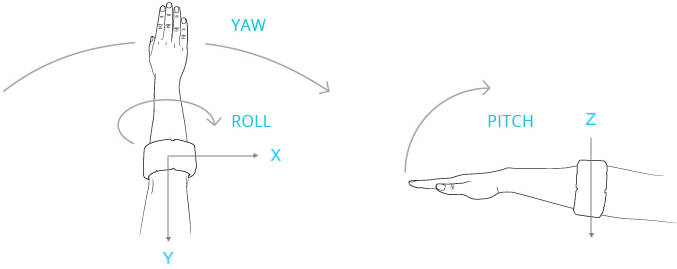
\includegraphics[width=0.7\linewidth]{pictures/myo}
	\caption{Myo Reference Frame (Source: http://developerblog.myo.com/gui-without-g-going-beyond-screen-myotm-armband/)}
	\label{fig:myo}
\end{figure}


\subsection{Data Processing}
\label{sec:Approach:Data-Processing}
The data from the acceleration, gyroscope, and EMG sensors needs to be processed in order to reduce noise and motion artifacts. Accelerometer and gyroscope data is smoothed using a $4^{th}$ order Butterworth band-pass filter with cut-off frequencies at 0.2Hz and 15Hz \cite{1419604}. The EMG data is high-pass filtered at 20Hz to reduce motion artifacts, as recommended in related works \cite{DeLuca2010}.

\subsection{Feature Extraction}
\label{sec:Approach:Feature-Extraction}
Human activity recognition systems take features extracted from processed data as input. The features are calculated through the use of a sliding window. Due to time it takes to perform different anatomical movements, the window size will have a length of 2s \cite{Dorfmeister2014}. The window will have a 50\% overlap, which has been proven sufficient in related work \cite{Wannenburg2016}. Table \ref{tab:features} displays all calculated features: Mean, standard deviation, and signal magnitude area for the IMU; Mean, signal magnitude area, root mean squared, and power spectral density for EMG.
\begin{table}[h]
	\centering
	\begin{tabular}{c|l|l}
		& \multicolumn{1}{l|}{Domain} & \multicolumn{1}{c}{Features} \\
		\hline
		\parbox[t]{2mm}{\multirow{3}{*}{\rotatebox[origin=c]{90}{IMU}}} & Time & Mean\\
		&& Standard deviation\\
		&& Signal Magnitude Area\\
		\hline
		\parbox[t]{2mm}{\multirow{3}{*}{\rotatebox[origin=c]{90}{EMG}}} & Time & Mean\\
		&& Signal Magnitude Area \\
		&& Root Mean Squared \\
		& Frequency & Power Spectral Density \\
	\end{tabular}
	\caption{Features for the Machine Learning algorithm}
	\label{tab:features}
\end{table}
\emph{Mean acceleration}, given in Equation \ref{eq:mean_acc}, is calculated by excluding the highest and lowest 10\% of the data, taking the sum of each of the three accelerometer axes and dividing by the number of values \cite{Totty2017}. Excluding the outliers removes any spikes that may occur due to collisions. The mean acceleration is calculated as $ \overline{acc}^{axis} $, where $axis$ represents all three axis $x,y,z$ and $N$ is the number of acceleration values. The values for $acc^{axis}_i$ include the data for an entire procedure, excluding the highest and lowest 10\%.
\begin{equation}\label{eq:mean_acc}
\overline{acc}^{axis} = \frac{1}{N}\sum_{i=1}^{N}acc^{axis}_i
\end{equation}
The mean acceleration feature was chosen to represent the quantity of motion \cite{Arif2015}.
\emph{Acceleration Standard deviation}, given in Equation \ref{eq:sd_acc}, is a measure describing the variance in a set of axis values. The calculated value is represented as $acc\_\sigma^{axis}$, where $axis$ represents all three axis $x,y,z$ and $N$ is the number of acceleration values.
\begin{equation}\label{eq:sd_acc}
acc\_\sigma^{axis} = \sqrt{\frac{\sum_{i=1}^{N}(acc^{axis}_i - \overline{acc}^{axis})}{N - 1}}
\end{equation}
\emph{Acceleration signal magnitude area} $acc\_sma$, given in Equation \ref{eq:sma_acc}, is computed by dividing the numerically-integrated area under the curve by the duration of the signal \cite{Totty2017}. The value of the axis are $acc_x,acc_y,acc_z$ respectively, and $T$ is the time duration of the signal.
\begin{equation}\label{eq:sma_acc}
acc\_sma = \frac{1}{T}\int_{0}^{T}(|acc_x|+|acc_y|+|acc_z|)dt
\end{equation}
The signal magnitude area of the acceleration feature was chosen, because it represents the gross motion of movements and the energy expenditure \cite{Jeran2016}. \emph{Mean angular rate of change}, given in Equation \ref{eq:mean_gyro}, is calculated by taking the sum of each of the three gyroscope axis $yaw, pitch, roll$ and dividing by the number of values $N$ \cite{Totty2017}.
\begin{equation}\label{eq:mean_gyro}
\overline{gyro}^{axis} = \frac{1}{N}\sum_{i=1}^{N}gyro^{axis}_i
\end{equation}
The mean rate of change feature was chosen, because it represents the quantity of rotation.
\emph{Rate of change standard deviation}, given in Equation \ref{eq:sd_gyro}, is a measure describing the variance in a set of axis values. The calculated value is represented as $gyro\_\sigma^{axis}$, where $axis$ represents all three axis $yaw,pitch,roll$ and $N$ is the number of acceleration values.
\begin{equation}\label{eq:sd_gyro}
gyro\_\sigma^{axis} = \sqrt{\frac{\sum_{i=1}^{N}(gyro^{axis}_i - \overline{gyro}^{axis})}{N - 1}}
\end{equation}
\emph{Angular rate of change signal magnitude area}, given in Equation \ref{eq:sma_gyro}, is calculated by dividing the numerically-integrated area under the curve by the duration of the signal \cite{Totty2017}. The value of the axis are $gyro_{yaw},gyro_{pitch},gyro_{roll}$ respectively, and $T$ is the time duration of the signal.
\begin{equation}\label{eq:sma_gyro}
gyro\_sma = \frac{1}{T}\int_{0}^{T}(|gyro_{yaw}|+|gyro_{pitch}|+|gyro_{roll}|)dt
\end{equation}
The angular rate of change signal magnitude area feature was chosen, because it represents the gross rotation of movements.
\par \emph{Mean muscle activation} $\overline{emg}^{channel}$, given in Equation \ref{eq:mean_gyro}, is calculated by taking the sum of each of the eight EMG channels and dividing by the number of values $N$.
\begin{equation}\label{eq:mean_emg}
\overline{emg}^{channel} = \sum_{i=1}^{N}emg^{channel}_i
\end{equation}
The mean muscle activation feature was chosen, because it represents the quantity of muscle movement.
\emph{Muscle activation signal magnitude area}, given in Equation \ref{eq:sma_emg}, is calculated by dividing the numerically-integrated area under the curve by the duration of the EMG signal. The EMG channels are represented as $e1,\dots,e8$ and $T$ is the time duration of the signal.
\begin{equation}\label{eq:sma_emg}
emg_{sma} = \frac{1}{T}\int_{0}^{T}(|e1|+|e2|+|e3|+|e4|+|e5|+|e6|+|e7|+|e8|)dt
\end{equation}
\emph{Muscle activation root mean squared} is calculated for each of the eight EMG channels and then averaged. Equation \ref{eq:rms_emg1} calculates the root mean squared for every channel $i=1,\dots,8$, where $N$ represents the number of values. Equation \ref{eq:rms_emg2} calculates the final averaged root mean squared value of all channels.
\begin{equation}\label{eq:rms_emg1}
emg\_channel\_i_{rms} = \sqrt{\frac{1}{N}(emg\_channel\_i_1^2+emg\_channel\_i_2^2+\dots+emg\_channel\_i_N^2)}
\end{equation}
\begin{equation}\label{eq:rms_emg2}
root\_mean\_squared = \frac{1}{8}\sum_{i=1}^{N}emg\_channel\_i_{rms}
\end{equation}
Root mean squared is proven to be the gold standard for EMG-force analysis \cite{KALLENBERG2008780}. The root mean squared value represents physiological activity during contraction of the muscle \cite{Totty2017}.
\emph{EMG Fast Fourier transformation} is applied to each EMG channel to transform the signal from the time domain into the frequency domain. Power Spectral Density represents the distribution of signal strength, which is taken from the frequency domain. The frequency spectrum can be used to detect muscle fatigue, force production and muscle fiber signal conduction velocity \cite{Gler2005}.
\subsection{Machine Learning}
\label{sec:Approach:Machine-Learning}
The machine learning algorithm approach trains a separate Hidden Markov Model (HMM) for every EMS procedure. HMMs in human activity recognition are based on modeling human activity as first-order Markov chains. A Markov chain represents a discrete time stochastic process covering a finite number of states, where the current state depends on the previous state \cite{Faicel2013}. Every coarse-grained movement is represented by a state for EMS procedures, while one HMM model corresponds to the procedure. The Figure \ref{fig:HMM} shows how each procedures is divided into its coarse-grained movement as state for the HMM.
\begin{figure}
	\centering
	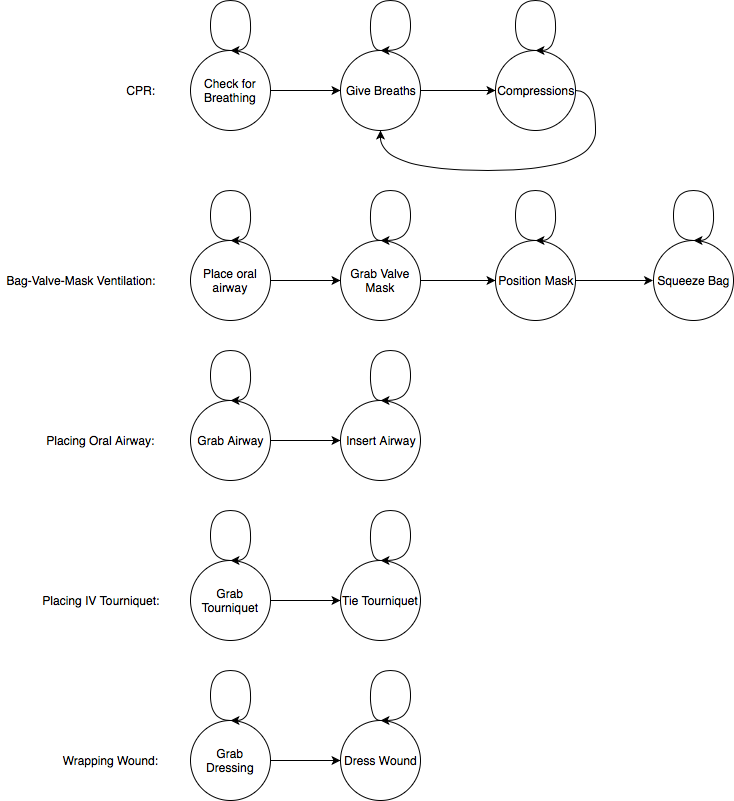
\includegraphics[width=0.7\linewidth]{pictures/HMM}
	\caption{HMM state diagram for EMS procedures}
	\label{fig:HMM}
\end{figure}
An observation sequence is tested by putting the data into each model and calculating the likelihood of the observation. The model with the highest likelihood is the class for the observation. A HMM $\lambda$ is represented as $\lambda = (A; B; \pi)$, where $A$ is the transition matrix, $B$ is the observation matrix, and $\pi$ is the initial probability array. $S$ is the state alphabet set in this case hidden, and $V$ is the observation alphabet set, such as the data we collect from the sensors \cite{Cheng2017}.
$$S=(s_1,s_2,\dots,s_N)$$
$$V=(v_1,v_2,\dots,v_M)$$
$Q$ is the fixed state sequence, and $O$ is the corresponding observation.
$$Q=q_1,q_2,\dots,q_T$$
$$O=o_1,o_2,\dots,o_T$$
$A$ is the transition matrix containing the probability of state $j$ following state $i$.
$$A = \{a_{ij} = P[q_t=s_j|q_t=s_i]\}, 1\leq i, j\leq M, \sum_{j=1}^{N}a_{ij}=1$$
$B$ is the observation matrix containing the probability of observation $k$ being produced from the state $j$.
$$B= \{b_{jk}=P[o_t=v_k|q_t=s_j]\}, \sum_{k=1}^{M}b_{jk}=1$$
$\pi$ is the initial probability array.
$$\pi=[\pi_i],\pi=P(q_1=s_i)$$
HMMs can be trained in two different ways: unsupervised and supervised. Supervised training is done, when a dataset is given with labels corresponding to every state of a HMM. The training data is labeled according to the EMS procedures to differentiate between the different HMMs. The HMMs are trained unsupervised with a predetermined number of states determined by from the Hierarchical Task Analysis using the Baum-Welch algorithm. The Baum-Welch algorithm is a strict version of the Expectation-Maximization algorithm, meaning the Baum-Welch algorithm is guaranteed to converge to at least a local maximum \cite{baum1970}. The output of the Baum-Welch algorithm is the most likely hidden transition probabilities $A$ and the most likely set of emission probabilities $B$. The modeled HMMs $\lambda_{j}$ for the EMS procedures $j=1,\dots,5$. Given a test sequence, $Y$, the probability for every HMM is calculated as follows:
$$P_j=\log(P(Y|\lambda_)), j=1,\dots,5$$
The result of the classification is taking the highest probability of all HMMs:
$$\lambda^\star=\max_{j}\{P(Y|\lambda_{j})\}$$

\section{Experimental Design}
\label{sec:Experimental-Design}
A machine learning algorithm needs data from different people performing all five procedures a number of times in order to be trained. The following chapter describes a study design to collect data from participants for the automatic recognition system. 

\subsection{Data Collection}
\label{sec:Experimental-Design:Data-Collection}
The study was designed to be within-subjects and consists of two questionnaires, training, and data collection. The first questionnaire asks for the participants demographics, such as: age, gender, education, handedness, and the amount of exercise per week. The second questionnaire evaluates the participants fatigueness, such as: the amount of caffeine intake, hours of sleep the last night, hours of sleep the night before, feeling of fatigue as Likert scale, and feeling of stress as Likert scale. The study is split into three days and structured as follows:
\begin{enumerate}
	\item \textbf{Day 1} (1 hour): First, the participant was asked to sign the consent form. Then, after a brief introduction to the experiment, the participant was fitted with two Myos on each of his or her arms. Next, the participant was asked to complete the demographic questionnaire, and the fatigue questionnaire. The remainder of the time, the participant was trained in the five medical procedures: CPR, wrapping a wound, tying a tourniquet, placing an oral airway, and bagging.
	\item \textbf{Day 2} (1 hour): After the participant was fitted with two Myos on each of his or her arms, he or she completed a fatigue questionnaire. For the remainder of the time, the participant was trained in the five medical procedures.
	\item \textbf{Day 3} (1 hour): After the participant was fitted with two Myos on each of his or her arms, he or she completed the fatigue questionnaire. For the first 15 mins, the participant was reminded of the training in the five medical procedures.
	After a five minute break the participant was asked to complete all five procedures for a minute each with 5 minute breaks in between each procedure, to reduce the impact of fatigue. Finally the participant was asked to do four rounds of completing all five procedures in a sequence: placing a tourniquet,  with a 5 minute break between each round.
\end{enumerate}

\subsection{Participant Demographics}
\label{sec:Data-Collection:Participant-Demographics}
The participant’s mean age was X (St. Dev. = X), where X\% were female and X\% were male. Most participants (X\%) completed an undergraduate degree, and the rest (X\%) have at least a high-school diploma. The participants were primarily right-handed (X\%), with Y\% left-handed. The participant's mean amount of exercise per week was X (St. Dev. = X).

\subsection{Machine Learning}
 The machine learning algorithm approach is compared to three different machine learning algorithms: SVM, decision-tree, and $k$-NN. SVMs work by constructing hyperplanes between classes. SVMs use different kernel functions to define the hyperplane, such as: linear, polynomial, and Gaussian radial basis function. The comparison will use the radial basis function, as the problem is non linear and it is the de facto standard. A decision-tree is a graph in which each node compares data values to a condition, a branch follows the result of the comparison, and each leaf is the class label. Finally, $k$-NN is an algorithm where the inputs are the $k$ closest neighbors of the data point. The algorithm counts the class label of each label and determines the label of the data point using majority voting. 
 
 \subsection{Research Questions}
 \label{sec:Data-Collection:Research-Questions}
 The evaluation of the automatic recognition system focuses on the accuracy of the machine learning algorithm, in order to evaluate two hypotheses:
 \begin{itemize}
 	\item $H_1$: Recognition of CPR and Bag-valve-mask ventilation will have the highest accuracy for each machine learning algorithm, due to its unique movements.
 	\item $H_2$: The recognition of a procedure through the sequence of fine-grained movements using a Hidden Markov Model will be more accurate than detecting through training coarse-grained movement models.
 \end{itemize}